\documentclass[a4paper,12pt]{report}

% Packages
\usepackage[utf8]{inputenc}  % Encoding
\usepackage{amsmath}         % Math symbols
\usepackage{amssymb}         % Additional math symbols
\usepackage{graphicx}        % Images
\usepackage[hidelinks]{hyperref}
\usepackage{caption}         % Captions
\usepackage{geometry}        % Page layout
\geometry{a4paper, margin=0.8in}
\usepackage{setspace}        % Line spacing
\usepackage{titlesec}        % Title customization
\usepackage{float}
\usepackage{listings}        % Code formatting
\usepackage{xcolor}
% Customization
\setcounter{secnumdepth}{3}  % Section numbering depth
\setcounter{tocdepth}{3}     % Table of contents depth
\setlength{\parindent}{0pt}
\renewcommand{\baselinestretch}{1.5}  % Line spacing

% Define Code Block Style
\lstdefinestyle{mystyle}{
    commentstyle=\color{gray},
    keywordstyle=\color{blue}\bfseries,
    stringstyle=\color{red},
    basicstyle=\ttfamily\footnotesize, % Change font to Courier New
    breaklines=true,                   
    captionpos=b,                      
    keepspaces=true,                   
    numbers=left,                      
    numbersep=5pt,                     
    numberstyle=\tiny\color{gray},     
    showspaces=false,                  
    showstringspaces=false,            
    showtabs=false,                    
    tabsize=4,
    frame=single % Clean single-line frame
}

% Apply the style globally
\lstset{style=mystyle}
\title{\textbf{Smart Home Automation}}
\author{Your Name}
\date{\today}

\begin{document}
\maketitle

\begin{abstract}
  Home automation using Raspberry Pi has gained popularity due to its low cost and capacity to improve convenience and energy efficiency.  This concept combines a smart home automation system with blockchain technology to enable safe and transparent energy invoicing.  The system gathers energy usage data from a smart energy meter linked to an Arduino and sends it to a cloud-based IoT platform via MQTT and REST APIs for real-time monitoring.This data is retrieved by a Web3 application, which then interacts with an Ethereum smart contract to securely produce and handle energy invoices.  Using blockchain technology, the system assures transparency, security, and decentralization in energy transactions.  The integration of IoT and smart contracts eliminates intermediaries, lowering operating costs and increasing efficiency.  This study exhibits a seamless transition from data collecting to invoicing and payment in a decentralized context, which helps to enhance smart energy management solutions.


\end{abstract}

\tableofcontents
\newpage

\chapter{Introduction}
Home automation using Raspberry Pi has gained popularity due to its numerous advantages and cost-effectiveness. These systems provide users with the ability to control household appliances through local networks or remote access, thereby enhancing convenience and energy efficiency\cite{jain2014raspberry}. 

Modern home automation technologies offer automatic meter reading, real-time monitoring, and remote control of electrical connections without the need for personal involvement\cite{chaudhari2017smart}.  The integration of Arduino controllers with GSM modules improves data transmission, allowing power companies to track energy use in kilowatt-hours (kWh) and create billing information\cite{rahman2015arduino}.

In addition to energy monitoring, home automation systems include sensors, cameras, and web-based applications to increase security and device control\cite{patchava2015smart}.  Real-time data gathering and storage in databases, such as MySQL, ensures accurate monitoring and analysis.  The use of the MQTT protocol improves data quality and dependability in IoT-based systems\cite{Atmoko_2017}.

Blockchain and smart contracts have emerged as disruptive technologies with the potential to transform many sectors.  Smart contracts are self-executing programs that autonomously enforce contractual conditions without the need for intermediaries, improving efficiency and lowering operational expenses\cite{10.1145/3328833.3328857}.  These technologies offer advantages such as transparency, security, and decentralization, making them appropriate for a wide range of applications, from identity management to business process automation\cite{chaudhari2017smart}.

 Home automation systems that combine IoT with blockchain-based smart contracts can improve trust and security in energy management.  This project investigates the integration of a smart energy meter with a blockchain-based billing system, using Raspberry Pi, IoT platforms, and Ethereum smart contracts to create a decentralized, transparent, and automated energy billing solution.


\chapter{Project Workflow}

\section{Overview}

This chapter depicts the workflow of a smart home automation system that is coupled with blockchain for energy billing.  The smart meter captures energy usage data, which is then transmitted to a cloud-based IoT platform for real-time monitoring\cite{jain2014raspberry}\cite{chaudhari2017smart}.  Data is processed using MQTT and REST APIs to ensure reliability\cite{Atmoko_2017}.

 A Web3 application obtains this information and communicates with an Ethereum smart contract to generate energy bills in a secure and transparent manner\cite{10.1145/3328833.3328857}\cite{Hu2018BlockchainbasedSC}.  By merging IoT and blockchain, the solution automates billing and payments, increasing efficiency and security.


\section{System Architecture}

The architecture consists of multiple interconnected components, including sensors, microcontrollers, cloud platforms, and blockchain technology. The data flow and interactions are illustrated in Figure~\ref{fig:workflow}.

\begin{figure}[h]
    \centering
    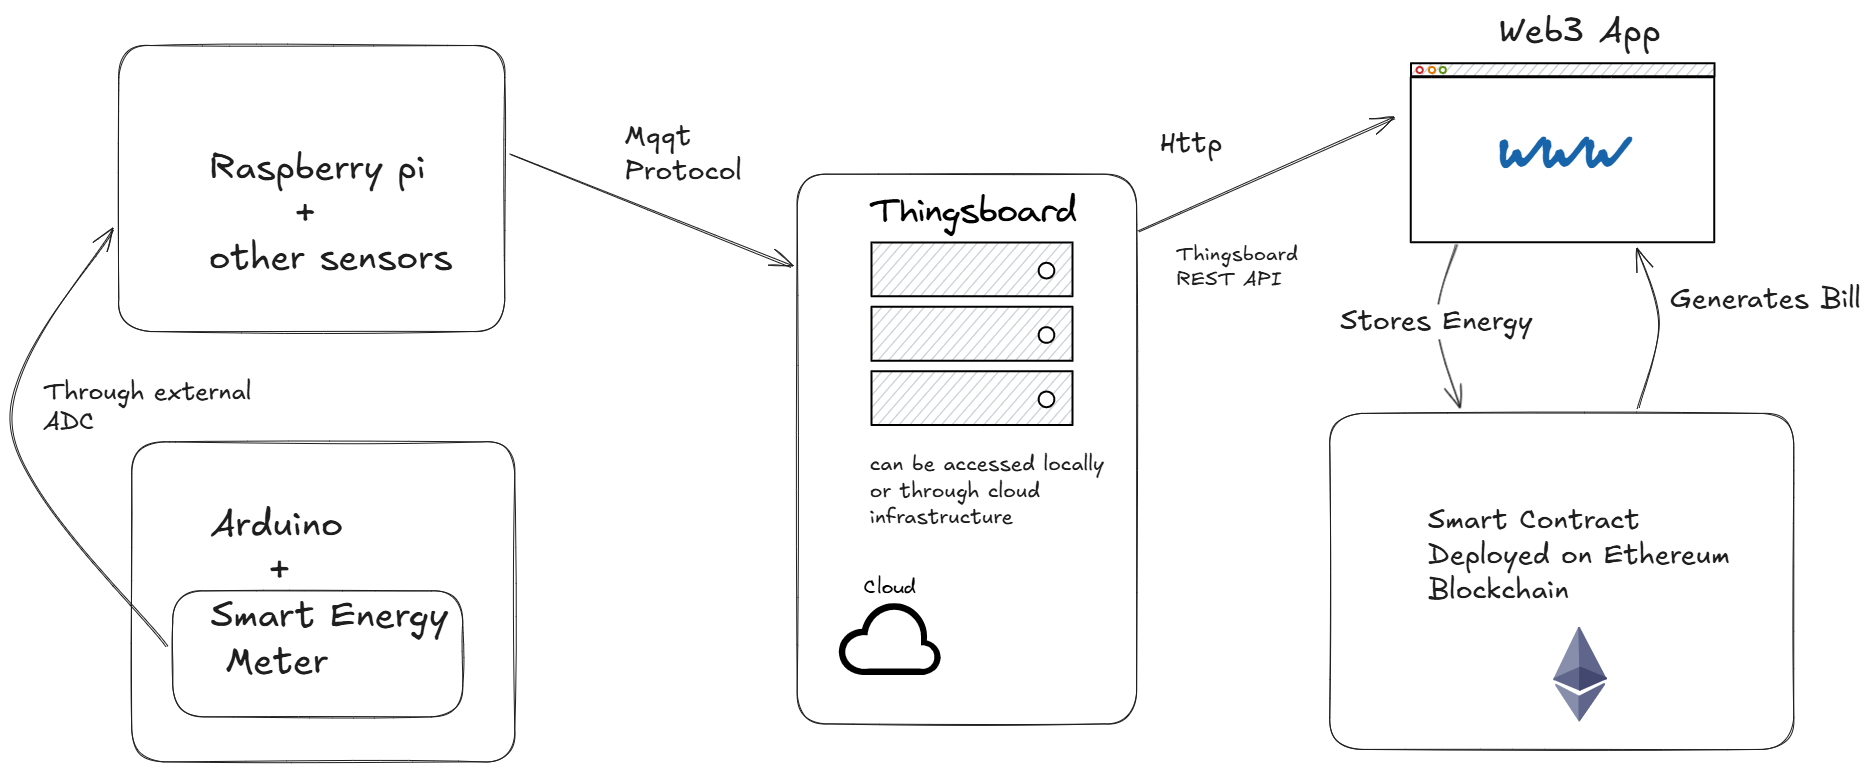
\includegraphics[width=0.9\textwidth]{basicArchitecture.png}
    \caption{System Workflow}
    \label{fig:workflow}
\end{figure}

\section{Components and Data Flow}

\subsection{Energy Measurement and Data Acquisition}

The system starts with an Arduino connected to a smart energy meter, which measures power consumption. Since Arduino lacks a built-in analog-to-digital converter (ADC) with the required resolution, an external ADC is used for accurate readings. The measured data is then transmitted to a Raspberry Pi for further processing.

\subsection{Data Transmission and Storage}

This chapter illustrates the workflow of a smart home automation system that is integrated with blockchain for energy billing.  The system's goal is to collect energy consumption data, store it in a cloud-based IoT platform, and bill and pay using a Web3 application that interacts with an Ethereum blockchain smart contract.

\subsection{Web3 Integration and Smart Contracts}

A Web3 application fetches energy consumption data from ThingsBoard via HTTP requests. The retrieved energy data is then stored in a smart contract deployed on the Ethereum blockchain. The smart contract automatically generates an energy bill based on the stored consumption values.

\subsection{Billing and Payment System}

Using HTTP queries, a Web3 application retrieves energy usage data from ThingsBoard.  A smart contract that is implemented on the Ethereum blockchain then stores the energy data that has been recovered.  Using the saved consumption values, the smart contract automatically creates an energy bill.

\section{Conclusion}

This process combines blockchain, cloud computing, and the Internet of Things to produce an automated and decentralized energy billing system.  An effective and transparent billing procedure is made possible by the modular architecture, which facilitates smooth data flow from energy monitoring to smart contract interactions.


\chapter{Schematic Design and Simulation in Proteus}
\section{Circuit Design}
The circuit consists of:
\begin{itemize}
    \item Voltage and current sensors connected to ESP8266
    \item UART communication between ESP8266 and Raspberry Pi
\end{itemize}

\begin{figure}[H]
    \centering

    \caption{Schematic Diagram of the System}
\end{figure}


\chapter{ThingsBoard Integration}
\section{Introduction to ThingsBoard}
Rapid breakthroughs in semiconductor technology and wireless communication have resulted in the development of low-cost sensor-based devices, which serve as the foundation for the Internet of Things (IoT) ecosystem\cite{estrin1999next}.  These sensors produce massive volumes of data, demanding effective collection, processing, and management frameworks.  IoT platforms play an important role in managing this data by offering connectivity, security, data visualization, and analytics capabilities\cite{hammi2018iot}\cite{gazis2015survey}.  Among these platforms, ThingsBoard has emerged as an effective open-source solution for IoT data collecting and management.

ThingsBoard is a Java 8-based IoT platform that acts as a gateway for devices that communicate using MQTT\cite{kegenbekov2022using}, CoAP\cite{shelby2014rfc}, and HTTP\cite{yassein2016application}.  These protocols allow for lightweight communication between resource-constrained IoT devices and cloud services.  MQTT is a publish/subscribe protocol for small, low-power devices that enables efficient message exchange via a broker with varying Quality of Service (QoS) levels\cite{kegenbekov2022using}.  In contrast, CoAP is an UDP-based protocol designed for limited contexts, with lower overhead but lesser dependability than MQTT\cite{shelby2014rfc}.
One of ThingsBoard's key features is the ability to build rules and plugins for message processing.  Rules contain data filters, metadata enrichment processors, and action triggers that change messages into new formats before sending them to plugins.  This rule-based system supports basic data processing, including threshold-based notifications.  However, the technology does not automatically support complex data aggregation over time or across several devices\cite{hammi2018iot}.

 ThingsBoard allows you to configure alerts for both devices and assets, which improves real-time monitoring and event-based automation.  When aberrant situations are recognized, these alerts alert users or initiate automated replies.  Furthermore, the platform supports both lightweight communication protocols, such as MQTT and CoAP, and classic RESTful services\cite{shelby2014rfc}. 

 \section{Prerequisites for ThingsBoard MQTT Integration}

 Before integrating ThingsBoard with MQTT, ensure that the required software components are installed and configured correctly. The ThingsBoard platform must be running on either a local system or a cloud server. Although ThingsBoard has a built-in MQTT broker, an external broker such as Mosquitto can also be used if needed. 

 
 Additionally, MQTT communication requires appropriate network settings. Ensure that port \textbf{1883} is open for unencrypted communication. Each device must authenticate with ThingsBoard using an \textbf{Access Token}, which is assigned when the device is created in ThingsBoard.
 
 \section{Connecting ThingsBoard with MQTT}
 
 To send telemetry data to ThingsBoard using MQTT, follow these steps:
 
 \subsection{Step 1: Define Connection Parameters}
 The first step is to configure the MQTT connection by specifying the ThingsBoard host, access token, and MQTT port. Replace the \texttt{ACCESS\_TOKEN} with the token obtained from the ThingsBoard device.
 
 \begin{lstlisting}
 THINGSBOARD_HOST = "localhost"
 ACCESS_TOKEN = "dU6S0YIAPX5WwfmB3wUi"  # Replace with your actual token
 MQTT_PORT = 1883
 \end{lstlisting}
 
 \subsection{Step 2: Install and Import MQTT Library}
 After setting up the connection parameters, ensure that the \texttt{paho-mqtt} library is installed. This library is required to establish an MQTT connection. Once installed, import the necessary modules in the Python script.
 
 \begin{lstlisting}
 import paho.mqtt.client as mqtt
 import json
 \end{lstlisting}
 
 \subsection{Step 3: Create MQTT Client and Connect}
 The next step is to create an MQTT client instance and authenticate using the access token. The client must then connect to the ThingsBoard host on the specified port.
 
 \begin{lstlisting}
 client = mqtt.Client()
 client.username_pw_set(ACCESS_TOKEN)  # Use Access Token for authentication
 client.connect(THINGSBOARD_HOST, MQTT_PORT, 60)
 \end{lstlisting}
 
 \subsection{Step 4: Publish Sensor Data}
 Once connected, sensor data must be prepared in JSON format and published to the ThingsBoard MQTT topic. The following code snippet demonstrates how to send temperature and humidity data.
 
 \begin{lstlisting}
 telemetry_data = {"temperature": 25.5, "humidity": 60}
 client.publish("v1/devices/me/telemetry", json.dumps(telemetry_data))
 print("Data sent successfully!")
 client.disconnect()
 \end{lstlisting}
 
 \subsection{Step 5: Verify Data in ThingsBoard}
 After publishing the data, it is essential to verify whether ThingsBoard has received it. This can be done by navigating to the ThingsBoard UI and checking the \textbf{Latest Telemetry} section of the configured device.

 \section{Prerequisites for ThingsBoard API Integration}
 
 Before integrating ThingsBoard with the API, ensure that the required software and authentication mechanisms are set up properly. The ThingsBoard platform must be installed on a local system or a cloud server to facilitate communication. A REST client such as Postman or the \texttt{fetch} API in JavaScript is necessary for interacting with ThingsBoard’s API. Additionally, proper network access should be configured to allow API requests.
 
 To ensure security, ThingsBoard requires authentication via a JSON Web Token (JWT). The authentication process involves sending a username and password to ThingsBoard’s login API. Upon successful authentication, a token is generated, which must be included in all subsequent API requests. Without this token, ThingsBoard will deny access to its resources.
 
 \section{Connecting to ThingsBoard API}
 
 To fetch telemetry data from ThingsBoard, follow these steps:
 
 \subsection{Step 1: Generate Access Token}
 The first step is to authenticate with ThingsBoard and obtain an access token. This is done by sending a POST request to the authentication API with valid credentials. The request should be formatted in JSON, containing a username and password.
 
 \begin{lstlisting}
 POST http://localhost:9090/api/auth/login
 Content-Type: application/json
 
 {
     "username": "tenant@thingsboard.org",
     "password": "tenant"
 }
 \end{lstlisting}
 
 \subsection{Step 2: Extract JWT Token}
 Once the authentication request is processed, the API will return a response containing a JWT token. This token is essential for making authorized requests to ThingsBoard. The response will be in JSON format, and the token can be extracted from the \texttt{token} field.
 
 \begin{lstlisting}
 {
     "token": "eyJhbGciOiJIUzI1NiIsInR5cCI...",
     "refreshToken": "eyJhbGciOiJIUzI1NiIsIn..."
 }
 \end{lstlisting}
 
 \subsection{Step 3: Fetch Telemetry Data}
 After obtaining the authentication token, the next step is to retrieve telemetry data from a specific device. The device ID must be specified in the request URL, and the JWT token must be included in the request headers under the \texttt{X-Authorization} field. The following JavaScript code demonstrates how to fetch power telemetry data from a ThingsBoard device.
 
 \begin{lstlisting}
 const response = await fetch( 
     `http://localhost:9090/api/plugins/telemetry/DEVICE/0eb8ae80-ffe6-11ef-b36a-71656502eb9c/values/timeseries?keys=power`,
     {
         headers: { "X-Authorization": `Bearer ${thingsboardToken}` },
     }
 );
 const data = await response.json();
 console.log(data);
 \end{lstlisting}
 
 \subsection{Step 4: Process Response Data}
 Once the telemetry data is retrieved, it will be returned in JSON format. The response will contain key-value pairs representing the requested telemetry values. The received data can then be processed, displayed, or stored as needed, depending on the application requirements.
 \section{Conclusion}
 Integrating ThingsBoard with MQTT allows for efficient and secure real-time data transmission for IoT devices. By following the methods mentioned, devices can authenticate, publish telemetry data, and take advantage of ThingsBoard's monitoring and automation capabilities. This lightweight and scalable strategy improves IoT installations by providing consistent connectivity while also allowing for future enhancements such as encryption and improved data handling.

\chapter{Blockchain and Smart Contracts}
\section{Introduction to Solidity}
Solidity is the Ethereum smart contract language. Below is a basic example:
\begin{lstlisting}[language=python]
pragma solidity ^0.8.0;

contract EnergyBilling {
    uint public energyConsumed;

    function recordEnergy(uint _energy) public {
        energyConsumed = _energy;
    }
}
\end{lstlisting}

\section{Advantages of Blockchain for Billing}
\begin{itemize}
    \item Ensures transparency in transactions
    \item Provides security with immutable records
    \item Removes the need for third-party billing systems
\end{itemize}

\section{Ethereum Gas Estimation}
Smart contract transactions require gas. Example of estimating gas:
\begin{lstlisting}
web3.eth.estimateGas({ data: "0x600160..." })
\end{lstlisting}

\chapter{Local Ganache and Dockerized Ganache}
\section{Setting Up Local Ganache}
Ganache is used for local Ethereum blockchain simulation:
\begin{lstlisting}
ganache-cli -p 7545
\end{lstlisting}

\section{Running Ganache in a Docker Container}
To run Ganache in a container:
\begin{lstlisting}
docker run -d -p 8545:8545 trufflesuite/ganache-cli
\end{lstlisting}

\chapter{Building the Web3 Application}
\section{Fetching Energy Data from ThingsBoard}
Using Web3.js, the app retrieves energy data from ThingsBoard and sends it to the smart contract:
\begin{lstlisting}[language=python]
const web3 = new Web3("http://localhost:8545");
const contract = new web3.eth.Contract(abi, contractAddress);

async function sendEnergyData(energy) {
    await contract.methods.recordEnergy(energy).send({ from: accounts[0] });
}
\end{lstlisting}

\section{Deploying the Smart Contract}
Using Truffle, deploy the contract:
\begin{lstlisting}
truffle migrate --network development
\end{lstlisting}

\section{Transaction History Recording}
Each energy billing transaction is recorded on the blockchain for transparency.

\chapter{Dockerizing the Complete System}
\section{Creating a Docker Compose File}
To ensure all services run together in containers:
\begin{lstlisting}
version: '3'
services:
  thingsboard:
    image: thingsboard/tb-postgres
    ports:
      - "1883:1883"
      - "8080:8080"

  ganache:
    image: trufflesuite/ganache-cli
    ports:
      - "8545:8545"

  web-app:
    build: ./web
    ports:
      - "3000:3000"
    depends_on:
      - ganache
      - thingsboard
\end{lstlisting}

\chapter{Conclusion}
This project successfully integrates IoT, cloud, and blockchain technologies to create an automated and transparent energy billing system. Future enhancements include adding AI-based energy predictions and integrating real-world payments.

\newpage
% References
\renewcommand{\bibname}{References}

\bibliographystyle{IEEEtran}
\bibliography{references}

\end{document}


